\begin{center}
	{\textbf{CARGA Y DESCARGA DE UN CONDENSADOR}}
\end{center}
\section{Objetivo}
Investigar la curva de tensión de carga de un condensador, así como, los factores que afectan el índice carga/descarga y qué efecto tienen estos factores en el índice.
\section{Materiales}
\begin{itemize}
	\item Fuente de alimentación 0 - 12$V$/6$V$ DC/AC.
	\item Interruptor.
	\item Conmutador.
	\item Resistencia de 10 y 47 $K$ \textohm.
	\item Condensador electrolítico de 47 y 470$\mu F$, bipolar.
	\item Alambre en bloque de conexión.
	\item Cables de conexión rojo y azul.
	\item Multímetro.
	\item Cronometro.
	\item Tablero de conexión.  
\end{itemize}
\section{Fundamento Teórico}
El alumno vendrá estudiando los siguientes prototipos:
\begin{itemize}
	\item Carga y descarga de un condensador.
\end{itemize}
\section{Montaje}
\begin{itemize}
	\renewcommand{\theenumi}{\Alph{enumi}}
	\item \textbf{ Primer experimento:} Monte el circuito como se muestra en la figura 1 y 2. Selecciona el multímetro a escala de 10$V$ y ponga la llave selectora en posición 1.
	\begin{figure}[h]
		\centering
		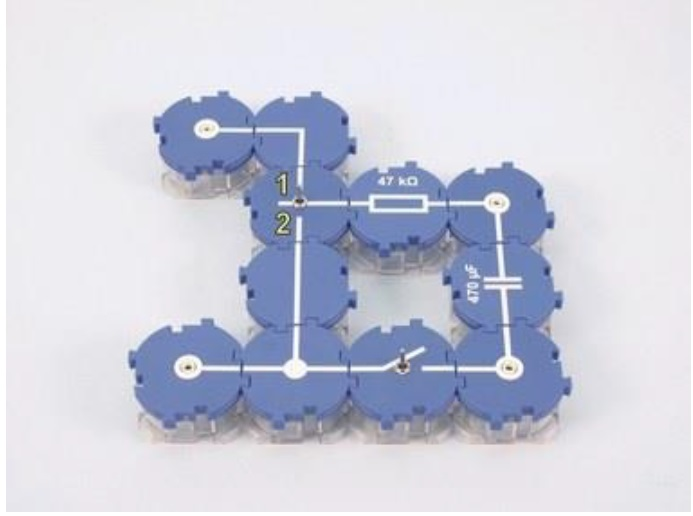
\includegraphics[width=5cm, height= 5cm]{imagenes/figura1}
		\caption{Primer circuito a montar}
	\end{figure}
	\begin{figure}[h]
		\centering
		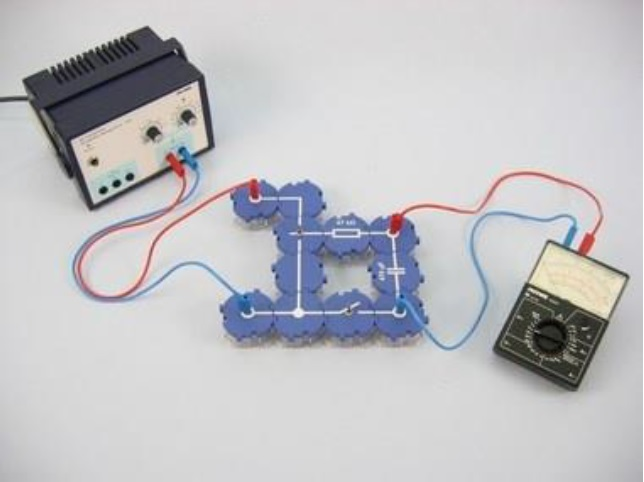
\includegraphics[width=5cm, height=5cm]{imagenes/figura2}
		\caption{Primer circuito siendo medido por un multímetro}
	\end{figure}
	\\
	\\
	\item \textbf{Segundo experimento:} Monte el circuito como se muestra  en la figura 3.
	\begin{figure}[h]
		\centering
		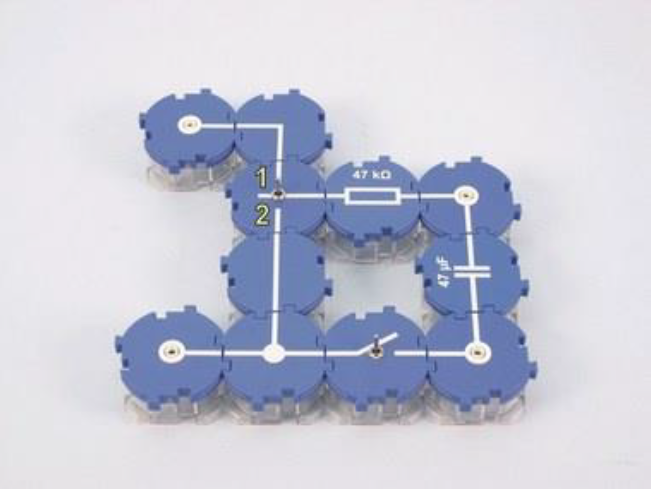
\includegraphics[width=5cm, height=5cm]{imagenes/figura3}
		\caption{Segundo circuito a montar}
	\end{figure}
\end{itemize}

\section{Procedimiento}
\textbf{Del primer experimento:}
\begin{itemize}
	\item Monte el experimento tal como se muestra en la figura  1. El interruptor debería estar en la posición de apagado y el conmutador se debería pulsa t a la posición 1. Seleccione ene voltímetro el rango de medición de 10$V$.
	\item Encienda la fuente de alimentación y fije la tensión directa a 10$V$.
	\item Cargue el circuito pulsando interruptor a la posición encendido y observe el voltímetro. Anote sus observaciones en (1).
	\item Descargue el circuito pulsando el conmutador a la posición 2. Observe el voltímetro  una vez más y anote su observación en (2).
	\item Cortocircuite el condensador por unos segundos usando un cable de conexión de 25cm. Retire el cortocircuito cuando la  tensión del condensador sea $U_{c}$ = 0$V$.
	\item Pulse el conmutador a la posición 1, iniciando en 0$V$. Mida la tensión $U_{c}$ del condensador en intervalos de 10 segundos. Anote en el cuadro 1.
\end{itemize}
\textbf{NOTA:} La toma de medidas requiere  una gran concentración y probablemente un poco de práctica. Si falla la primera serie de medidas, cortocircuite brevemente el condensador y repita las mediciones.
\begin{itemize}
	\item Pulse el conmutador a la posición 2 y tome las medidas de la tensión del condensador en intervalos de 10 segundos. Registre los valores en la tabla 1.
	\item Interrumpa la carga del circuito colocando el interruptor en la posición abierta.
\end{itemize}

\section{Observaciones y resultados de las mediciones}
\begin{itemize}
	\item \textbf{Primer experimento:} Observaciones hechas durante el experimento.
	\begin{enumerate}
		\item El experimento consto de un circuito conformado por un condensador de 470$\mu F$, una resistencia de 10$K$\textohm, un interruptor y una fuente de alimentación continua de 12$V$. En la cual se pudo observar el  proceso de carga de una condensador y también se llego a recopilar los datos que se muestran en el siguiente cuadro. 
		\item
	\end{enumerate}
	\begin{table}[h]
		\begin{center}
			\begin{tabular}{|c|c|c|c|c|c|c|c|c|c|c|c|c|c|}
				\hline
				Carga: $U_{c}/V$&0&1&2&3&4&5&6&7&8&9&10&11&12\\
				\hline
				$t_{1}/s$&0&3&5&7&10&14&18&24&29&37&49&72&118\\
				\hline
				$t_{2}/s$&0&3&5&8&11&15&19&24&30&36&50&72&113\\
				\hline
				$t_{3}/s$&0&2&4&8&11&16&20&27&35&47&69&74&111\\
				\hline
				\textbf{$t_{promedio}/s$}&0&3&5&8&11&15&19&25&31&40&56&73&114\\
				\hline
			\end{tabular}
		\caption{Resultados del primer experimento}
		\end{center}
	\end{table}
\end{itemize}
\section{Cuestionario}
\begin{enumerate}
	\item \textbf{Usando los datos de carga y descarga del cuadro 1, trace un gráfico.}
	\begin{figure}[h]
		\centering
		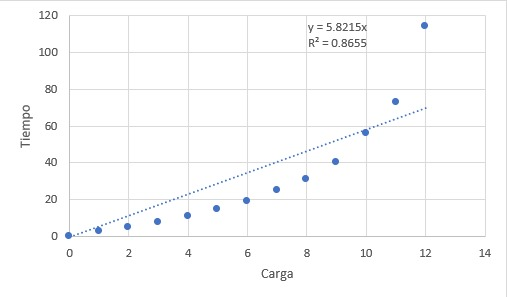
\includegraphics[height= 8cm, width=12cm]{imagenes/grafico}
		\caption{Grafica carga del condensador versus el $t_{promedio}$ de carga}
	\end{figure}
	\item \textbf{Explique la curva de estos gráficos y/o sus observaciones anotadas en 1:}\\
	La gráfica muestra una curva creciente, lo que nos indica que existe una relación directamente proporcional entre el tiempo y la carga del condensador puesto que si la carga aumenta el tiempo también aumentará. Esto teniendo en cuenta que en el experimento realizado se observó que para que el condensador tenga mayor voltaje transcurre un mayor tiempo. Asimismo gracias al valor del coeficiente de correlación 0.8655  podemos confirmar la fuerte relación de ambas variables
	\item \textbf{Explique la relación entre el tiempo que toma cargar un condensador y la capacidad $C$, así como la relación entre el tiempo necesario para cargar y la resistencia $R$ (designado como una resistencia de carga). Explique por qué debe ser así la relación:\\}
	El tiempo de carga es directamente proporcional a la capacitancia de un condensador, si y solo si el condensador todavía no llega a su capacitancia máxima. \\
	Se sabe que una resistencia se opone al flujo de la corriente eléctrica, por lo que la cantidad de corriente que llegué al condensador será menor, siendo así que el condensador demoré más tiempo en  realizar la carga a su máxima. Esto nos da a entender que el tiempo de carga en un condensador sera directamente proporcional a la resistencia.	\\
	El tiempo de carga del condensador es proporcional al valor de R y de C. Multiplicando el valor de la resistencia por la capacidad obtenemos lo que se denomina constante de tiempo.
	$t = R.C $\\
	Donde:
	\begin{itemize}
		\item $t$: es la constante de tiempo.
		\item $R$: es la resistencia.
		\item $C$: es la capacidad del condensador.
	\end{itemize}
\end{enumerate}